\documentclass{beamer}
\usetheme{metropolis}
\usepackage{solarized-light}
\usepackage{graphicx}
\usepackage{listings}
\usepackage{svg}
\usepackage{amsmath}
\usepackage{float}
\usepackage{fontspec}
\usepackage{microtype}
% we need to define this because otherwise listings won't
% pick up style changes
\newfontface\UMono[Scale=MatchUppercase]{UbuntuMono}
\setmonofont[Ligatures=TeX]{UbuntuMono}

\makeatletter
\lst@InstallKeywords k{attributes}{attributestyle}\slshape{attributestyle}{}ld
\makeatother

\lstdefinestyle{cpp}{
  language=C++,
  basicstyle=\fontsize{7}{7}\UMono,
  morecomment=[l][\color{sorange}]{\#},
  moreattributes={main},
  attributestyle = \color{sblue},
  literate={
    {-}{{-}}1
  }
}

\lstdefinestyle{shell}{
  basicstyle=\fontsize{6}{6}\UMono,
  literate={
    {-}{{-}}1
  }
}

\lstdefinestyle{gtest}{
  basicstyle=\fontsize{7}{7}\UMono,
  alsoletter=\[\=\]\-,
  literate={
    {--}{{-\,-}}2
    {[==========]}{{\textcolor{mysgreen}{[==========]}}}{10}
    {[----------]}{{\textcolor{mysgreen}{[----------]}}}{10}
    {[\ RUN\ \ \ \ \ \ ]}{{\textcolor{mysgreen}{[ RUN\ \ \ \ \ \ ]}}}{10}
    {[\ \ \ \ \ \ OK\ \ ]}{{\textcolor{mysgreen}{[\ \ \ \ \ \ OK\ \ ]}}}{10}
  }
}

\newcommand{\mytitle}{Property based testing in C++}

\title{\mytitle}
\subtitle{How to write 1000s of tests in one sitting?}
\author{Patryk Ma\l{}ek}
\institute{\footnotesize\url{https://github.com/pmalek}}
\date{}

\setbeamertemplate{frame footer}{\tiny\mytitle}
\setbeamersize{text margin left=20pt,text margin right=20pt}

\setlength{\leftmargini}{8pt}

%==============================================================
%==============================================================
%==============================================================

\begin{document}

  \maketitle

%==============================================================

\begin{frame}[fragile]{Let's talk about tests}

\begin{uncoverenv}<+->
Suppose we have the following \texttt{add} function signature:
\begin{lstlisting}[style=cpp]
int add(int x, int y);
\end{lstlisting}
\end{uncoverenv}

\begin{uncoverenv}<+->
How would you approach testing it?
\end{uncoverenv}

\begin{uncoverenv}<+->
\begin{lstlisting}[style=cpp]
TEST(AddTest, OnePlus3Equals4){
  EXPECT_EQ(4, add(1,3));
}
\end{lstlisting}
\end{uncoverenv}

\begin{uncoverenv}<+->
\begin{lstlisting}[style=cpp]
TEST(AddTest, OnePlus0Equals1){
  EXPECT_EQ(1, add(1,0));
}
\end{lstlisting}
\end{uncoverenv}

\begin{uncoverenv}<+->
\begin{lstlisting}[style=cpp]
TEST(AddTest, OnePlusMinus1Equals0){
  EXPECT_EQ(0, add(1,-1));
}
\end{lstlisting}
\end{uncoverenv}

\begin{uncoverenv}<+->
\begin{lstlisting}[style=cpp]
TEST(AddTest, BigNumbersAreCorrectlyAdded){
  EXPECT_EQ(186321, add(87556,98765));
}
\end{lstlisting}
\end{uncoverenv}

\end{frame}

%==============================================================

\begin{frame}[fragile]{Let's talk about tests}

\begin{uncoverenv}<+->
What if the implementation looked like...
\end{uncoverenv}

\begin{uncoverenv}<+->
... this
\begin{lstlisting}[style=cpp]
int add(int x, int y){
  if( x == 7 ) return 1;
  return x + y;
}
\end{lstlisting}
\end{uncoverenv}

\begin{uncoverenv}<+->
ehh ...
\end{uncoverenv}

\end{frame}

%==============================================================

\begin{frame}[fragile]{How do you define a good test?}

\begin{uncoverenv}<+->
How can we test addition?
\end{uncoverenv}

\begin{uncoverenv}<+->
Let's think about its properties
\end{uncoverenv}

\begin{itemize}[<+->]

\item Commutativity:
\begin{lstlisting}[style=cpp]
Test: "result shouldn't depend on order of parameters"
    int x = random int
    int y = random int
    ASSERT(add(x,y) == add(y,x))
\end{lstlisting}

\item Identity:
\begin{lstlisting}[style=cpp]
Test: "adding 0 to any number yields the same number"
    int x = random int
    ASSERT(add(x,0) == x)
\end{lstlisting}

\item Associativity:
\begin{lstlisting}[style=cpp]
Test: "result shouldn't depend on order of operations"
    int x = random int
    int y = random int
    int z = random int
    ASSERT(add(z,add(x,y)) == add(add(x,y),z))
\end{lstlisting}

\end{itemize}

\end{frame}

%==============================================================

\begin{frame}[fragile]{RapidCheck}

\begin{minipage}{\textwidth}
\begin{center}
  \scriptsize{\url{https://github.com/emil-e/rapidcheck}}
  
\includegraphics[width=10pt]{octo}
\end{center}
\end{minipage}

\begin{figure}
  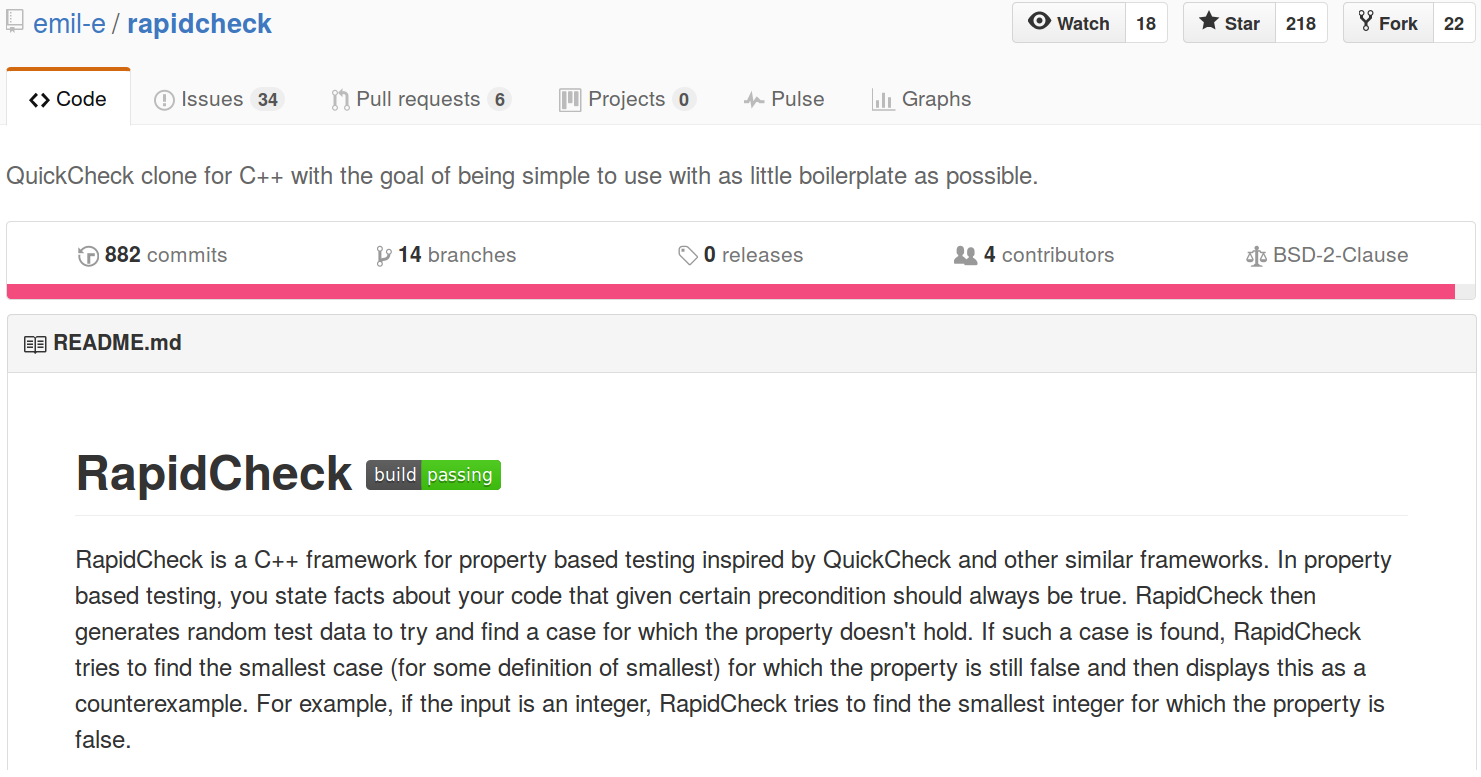
\includegraphics[width=\textwidth]{rapidcheck.png}
\end{figure}

\end{frame}

%==============================================================

\begin{frame}[fragile]{RapidCheck addition tests}

Let's use \texttt{RapidCheck} with our examples:

\begin{lstlisting}[style=cpp]
#include <rapidcheck.h>

int main() {
  rc::check("result shouldn't depend on order of parameters",
            [](int x, int y){
    RC_ASSERT( add(x,y) == add(y,x) );
  });

  rc::check("adding 0 to any number yields the same number",
            [](int x){
    RC_ASSERT( add(x,0) == x);
  });

  rc::check("result shouldn't depend on order of operations",
            [](int x, int y, int z){
    RC_ASSERT( add(z, add(x,y)) == add(add(x,y), z));
  });
}
\end{lstlisting}

\end{frame}

%==============================================================

\begin{frame}[fragile]{RapidCheck output}

Output we might expect on failure:

\begin{lstlisting}[style=shell]
Using configuration: seed=1313473344045799863

- result shouldn't depend on order of parameters
Falsifiable after 18 tests and 1 shrink

std::tuple<int, int>:
(7, 0)

/home/patryk/workspace/git/rapidcheck_cmaketest/src/main.cpp:43:
RC_ASSERT(add(x,y) == add(y,x))

Expands to:
1 == 7

- adding 0 to any number yields the same number
Falsifiable after 18 tests

std::tuple<int>:
(7)

/home/patryk/workspace/git/rapidcheck_cmaketest/src/main.cpp:48:
RC_ASSERT(add(x,0) == x)

Expands to:
1 == 7

...
\end{lstlisting}

\end{frame}

%==============================================================

\begin{frame}[fragile]{RapidCheck output}

\begin{uncoverenv}<+->
After fixing our implementation like so:
\begin{lstlisting}[style=cpp]
int add(int x, int y){
  return x + y;
}
\end{lstlisting}
\end{uncoverenv}

\begin{uncoverenv}<+->
All the tests pass:
\begin{lstlisting}[style=shell]
Using configuration: seed=1912891779374620633

- result shouldn't depend on order of parameters
OK, passed 100 tests

- adding 0 to any number yields the same number
OK, passed 100 tests

- result shouldn't depend on order of operations
OK, passed 100 tests
\end{lstlisting}
\end{uncoverenv}

\end{frame}

%==============================================================

\begin{frame}<1>[label=rapidcheck_configuration]
\frametitle{RapidCheck configuration}

\texttt{RapidCheck} has a lot of configuration options:

\begin{itemize}[<+- | alert@+>]
\item \texttt{googletest}/\texttt{Boost.Test} integration
\item "shrinking"
\item Reproducible failures/seed
\item Generators for user defined types
\item Built in support for many STL types
\item Configurable number of tests to run
\item ... and many more
\end{itemize}

\end{frame}

%==============================================================

\begin{frame}[fragile]{Google test integration}

You can integrate \texttt{RapidCheck} with google test:

\begin{lstlisting}[style=cpp]
#include <gtest/gtest.h>
#include <rapidcheck.h>
#include <rapidcheck/gtest.h>

RC_GTEST_PROP(TestCase, inRange, (int first, int second))
{
  int x = *rc::gen::inRange(first, second);
  RC_ASSERT(x >= first);
  RC_ASSERT(x < second);
}

int main(int argc, char **argv)
{
  ::testing::InitGoogleTest(&argc, argv);
  return RUN_ALL_TESTS();
}
\end{lstlisting}

\end{frame}

%==============================================================

\begin{frame}[fragile]{Google test integration}

And you get familiar output:

\begin{lstlisting}[style=gtest]
[==========] Running 1 test from 1 test case.
[----------] Global test environment set-up.
[----------] 1 test from TestCase
[ RUN      ] TestCase.inRange
Using configuration: seed=4574822431460607532
[      OK  ] TestCase.inRange (32 ms)
[----------] 1 test from TestCase (33 ms total)

[----------] Global test environment tear-down
[==========] 1 test from 1 test case ran. (33 ms total)
\end{lstlisting}

\end{frame}

%==============================================================

\againframe<2>{rapidcheck_configuration}

%==============================================================

\begin{frame}[fragile]{shrinking}

\begin{uncoverenv}<+->
Suppose we have the following output:
\begin{lstlisting}[style=shell]
Using configuration: seed=1313473344045799863

- all numbers in vector have desired value
Falsifiable after 100 tests

std::vector<int>:
[-2319, 12, -223584, -2071, 4383, -3727, -7431, -123897]
\end{lstlisting}
\end{uncoverenv}

\begin{uncoverenv}<+->
Is it clear what might be wrong with our implementation?
\end{uncoverenv}

\begin{uncoverenv}<+->
How about now?
\begin{lstlisting}[style=shell]
Using configuration: seed=1313473344045799863

- all numbers in vector have desired value
Falsifiable after 18 tests and 1 shrink

std::vector<int>:
[0, 0, 0, 0, 100, 0, 0, 0]
\end{lstlisting}
\end{uncoverenv}

\begin{uncoverenv}<+->
Implementation:
\begin{lstlisting}[style=cpp]
ASSERT(std::all_of(v.begin(), v.end(), [](int i){ return i<100; }));
\end{lstlisting}
\end{uncoverenv}

\end{frame}

%==============================================================

\againframe<3>{rapidcheck_configuration}

%==============================================================

\begin{frame}[fragile]{Reproducible failures}

Each time you get a failure with \texttt{RapidCheck} you'll get
a similar information in the end of console output:

\begin{lstlisting}[style=shell]
Some of your RapidCheck properties had failures. To reproduce these, run with:
RC_PARAMS="reproduce=C0SYkRWaudGIwACdvBSYulHIuVXbiVmcgkXalxGZzBCdoVGIzFWblBib11mYlJ3H+
35MMG+Aw_h_dODjhPA8f4fnzwY4DA_H+35MMG+AwDIIA0ADAAAAAEDchJXYtVGdlJ3cg8mckVmcgMGah52ZlBC
ZvV2cudCdgEmZmV2Y0BCdoVGIyV2c1xGdf4fnzwY4DA_H+35MMG+Aw_h_dODjhPA8f4fnzwY4DAPggAQDMAAAA
AA"
\end{lstlisting}

You can reproduce a failed test (with seed that was used to run
it) by running your test binary with \texttt{RC\_PARAMS}
environment variable.

\end{frame}

%==============================================================

\againframe<4->{rapidcheck_configuration}

%==============================================================


\begin{frame}{Conclusion}

\begin{center}

\uncover<+->{Think about your systems under test as fellow human beings}

\uncover<+->{Don't think about them in terms of input and output pairs}

\uncover<+->{Consider their properties and conditions that should hold}

\end{center}

\end{frame}

%==============================================================

\begin{frame}[fragile]{Examples source code}
\begin{center}
  Examples available at:

  \begin{figure}
  
\includegraphics[page=1,width=.05\textwidth]{octo}
  \end{figure}

  \url{https://github.com/pmalek/rapidcheck_codedive.git}
\end{center}

\end{frame}

%==============================================================

\appendix

\begin{frame}[allowframebreaks]{References}

  \bibliography{property_based_testing_cpp}
  \bibliographystyle{abbrv}

\end{frame}

%==============================================================

\begin{frame}[standout]
  Questions?
\end{frame}

%==============================================================

\end{document}
